\TODO
EHW: Evolvable hardware.
POE: Phylogeny, Ontogeny, Epigenesis \cite{sipper1997poe}.

Features: Graceful degradation, Robustness, Redundancy.

\TODO
Phylogeny, named after evolution of the species "Phylogeny" is temporal evolution due to mutation, reproduction.
Provides diverity for "survival of the fittest".
Ontogeny = development / cell division, a zygote replicates into a larger structure where each cell specializes.
Difficult to store each cell type/function.
Example: Human brain can't be specified by genome.
Epigenesis: Modification (learning) during the lifetime of the organism.

\TODO
Equivalent: Artificial Evolution, Artificial Development, Artificial Learning.
The two first are used in this thesis.

%==============================================================================%

\section{Artificial Evolution}

\TODO
NASA has high success in creating antennas \cite{hornby2006antenna}.
Robot controllers.
Platform for robot controller evolution \cite{haddow1999robot}.
Evolutionary Algorithms (EAs).

\subsection{Genetic Algoritmhs}

A genetic algorithm (GA) is a very common type of EA.
It represents each solution as a genotype, a binary string used as a blueprint to create the solution itself, called a phenotype.
The genotype is comparable to nature's DNA, and it is this genetic material which is modified in the evolutionary process.

\begin{figure}[!ht]
    \centering
    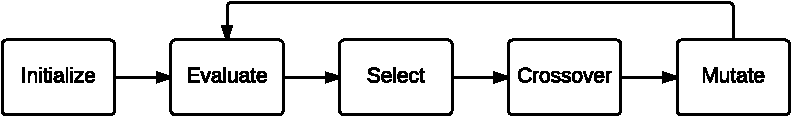
\includegraphics[width=0.9\textwidth]{ga}
    \caption[Genetic Algorithm]{
        A genetic algorithm.
        The cycle is broken when the fitness is above a given threshold.
    }
    \label{fig:ga}
\end{figure}

The GA process is shown in \figurename~\ref{fig:ga}.
First, a base population with random genotypes is generated.
Then, each phenotype is constructed and evaluated using a fitness function.
If a solution has a fitness score above a set threshold, the process stops.
Otherwise, a new population is created by selecting solutions with high fitness scores, crossing their genotypes, and mutating the results, before repeating the process.

\subsection{Evolution in Materio}
\todo{replace with EWH?}

\TODO
Embodiment principles.
Evolve in software, test in software.
Evolve in software, test in hardware.
Evolve and test in hardware.

%==============================================================================%

\section{Artificial Development}

\TODO
Attractors.
Adaptation.

\subsection{Lindenmayer Systems}

\TODO
\cite{prusinkiewicz1990lindenmayer}.
Lindenmayer: Biologist and Botanist.
System to describe the growth of plants.
Especially branching structure.
Start with an axiom.
Recursively build larger shapes by applying development rules.
Example: Sierpinski Triangle.
Used to generate plants and trees in media \CN.

%==============================================================================%

\section{Cellular Automata}

A cellular automaton (CA) is a computational structure made up of vast numbers of very simple functional elements called cells.
It is an attempt to mimic the structure found in biological lifeforms, where complex results emerge from interactions between many simple cells.
The key principles are massive parallelity, local interactions and simple computational units.
As seen in \figurename~\ref{fig:computing-principles}, this is the direct opposite paradigme of the general-purpose serial architecture that is common in computers today.
However, CAs have been shown to be Turing complete \cite{codd1968cellular, neumann1966selfreplication}, and can therefore perform the same tasks.

\begin{figure}[!ht]
    \centering
    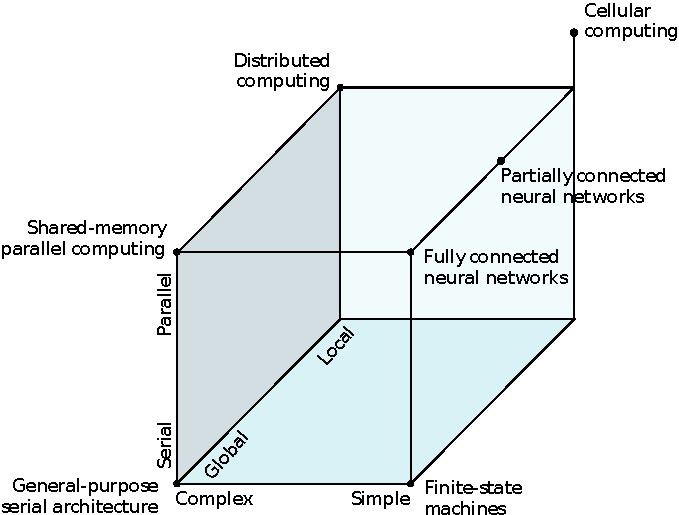
\includegraphics[width=0.85\textwidth]{computing-principles}
    \caption[Computing principles]{
        Graphical representation of how different computing paradigmes relate with regards to computing principles.
        (Reprinted from \cite{sipper1999emergence})
    }
    \label{fig:computing-principles}
\end{figure}

There are many variations of CAs, which are discussed in great detail in \cite{sipper1999emergence}.

\TODO
Computation by emergence.
Desired because of scalability and robustness.
Hard for humans to comprehend how to program.
Evolutionary often used.

\TODO
One of the greatest challenges with CAs is how to represent input and parse output.
Discrete Fourier Transform (DFT) is promising for analysis of output \cite{berg2013ca}.

\TODO
Here: Discrete, Deterministic, Synchronous, Non-uniform, Exhaustively Ennumerated CA with 3D von Neumann neighborhood.

\begin{itemize}
    \item Discrete vs Continuous values
    \item Exhaustive enumeration vs Parameterized vs others
    \item Synchronous vs asynchronous updates
    \item Uniform vs non-uniform tranfer functions
    \item Deterministic vs non-deterministic
    \item Direct programming vs Adaptive (evolution)
\end{itemize}

\TODO
Also possible to vary how cells are connected.
Connection pattern is called neighborhood.

\subsection{Neighborhoods}

\TODO
Lower dimensional CA can achieve the same as higher, if neighborhood is increased.

\begin{itemize}
    \item Regular grid vs graph
    \item 1D vs 2D vs 3D
    \item Full vs von Neumann
    \item Can include itself
\end{itemize}

\subsection{Complexity Classes}

\TODO
Wolfram: \cite{wolfram1984complexity}.
Lambda: Measure of how often transition function specifies a new state.
With increasing lambda: class 1, 2, 4, 3.
4 is the sweetspot.
Has structures that can store data, long cycles that can compute.

\begin{itemize}
    \item Class 1 - Uniform
    \item Class 2 - Repetitive patterns
    \item Class 3 - Chaos
    \item Class 4 - Complex (The edge of chaos)
\end{itemize}

%==============================================================================%

\section{FPGA}

A Field Programmable Gate Array (FPGA) is a type of reconfigurable hardware.
It can implement any desired logical operation by configuring and connecting a number of look-up tables (LUTs) and flip-flops (FFs).
FPGAs can also contain dedicated blocks for addition, multiplication, storage, and other functions.
These elements are grouped into configurable logic blocks (CLBs), which through a network of interconnects can be connected to each other or input/output pins.
An example of this structure is shown in \figurename~\ref{fig:fpga}.
Note that modern FPGAs consists of thousands of CLBs and hundreds of I/O pins \cite{ds160}.
\todo{mention DSP slices}

\begin{figure}[!ht]
    \centering
    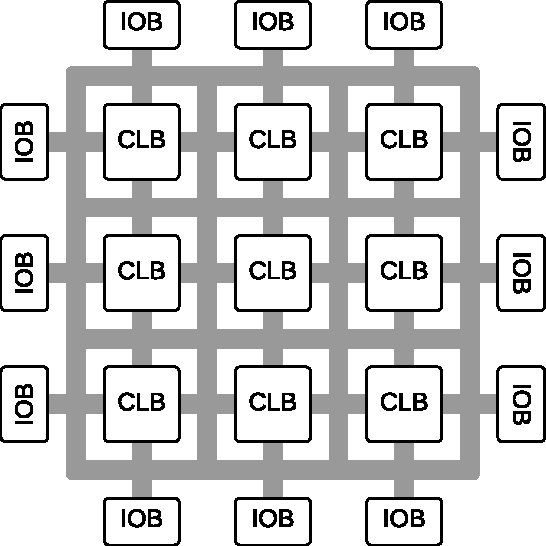
\includegraphics[width=0.60\textwidth]{fpga}
    \caption[FPGA]{
        High-level block diagram of an FPGA.
        An array of configurable logic blocks (CLBs) and input/output blocks (IOBs) are connected by a network of interconnects.
    }
    \label{fig:fpga}
\end{figure}

FPGAs have been the subject of EHW research due to their reconfigurability, and several researchers have been successful in evolving working electronic circuits \cite{huelsbergen1998evolution} \cite{thompson1997evolved}.
However, the resulting circuits have often ended up using intrinsic properties of the silicon and been very sensitive to environmental changes.

A problem with using modern FPGAs for EHW research is that some configuration bitstrings can destroy the FPGA by creating short-circuits \cite{ug380} \cite{xapp151}.
This means that the bitstrings can not be used directly as the genotype without complicated tests to discard those that are dangerous.

\subsection{Sblock}
\label{sec:sblock}

The sblock was introduced as part of a new EHW-friendly FPGA architecture in \cite{haddow2000sblock}.
The architecture is a non-uniform CA with a von Neumann neighborhood, where the update function of each cell is independently configurable at run-time.
The cells, known as sblocks, are very simple structures; they consist of a configurable look-up-table (LUT) and a flip-flop (FF), as shown in \figurename~\ref{fig:sblock}.

\begin{figure}[!ht]
    \centering
    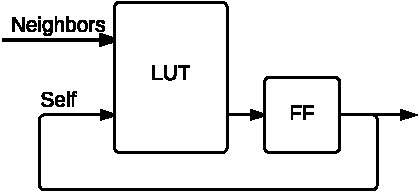
\includegraphics[width=0.5\textwidth]{sblock}
    \caption[Sblock]{
        Detailed block diagram of an sblock.
        The LUT can be reconfigured on-the-fly to implement any logical function.
    }
    \label{fig:sblock}
\end{figure}

The greatest benefit of using sblocks for EHW research is that there is no risk of damage or exploitation of intrinsic properties in the silicon.
Additionaly, the simple structure and hardwired signal routing allows for very efficient area usage.
The likelihood of a mass-produced sblock-FPGA arriving on the market in the near future is slim.
However, it is possible to implement it virtually within an other FPGA.

%==============================================================================%

\section{PCI Express}

The PCI Express interface was designed to tackle the arising trouble with clocked parallel buses like PCI.
The problem with such buses is that the clock speed can not be increased beyond a given threshold, as the slightly different lengths of the wires causes data to arrive at slightly different times.
Reducing the clock period to less than the variation in arrival time means the data will become corrupted.
This problem is exacerbated with increasing bus size.

PCI Express is therefore based on serial communication over differential pairs (lanes\footnotemark) without the need for a reference clock \cite{pcie}.
\footnotetext{
    PCI Express operates in full duplex mode, which means that each lane has an independent differential pair in each direction.
    1, 2, 4, 8, 16 or 32 lanes are supported, but data is striped and thus still transmitted serially.
}
This allows an extremely fast clock speed compared to a parallel bus, and much greater bandwidth in total.
PCI Express consists of three layers; the physical layer, the data link layer and the transaction layer, structured as shown in \figurename~\ref{fig:pcie}.

\begin{figure}[!ht]
    \centering
    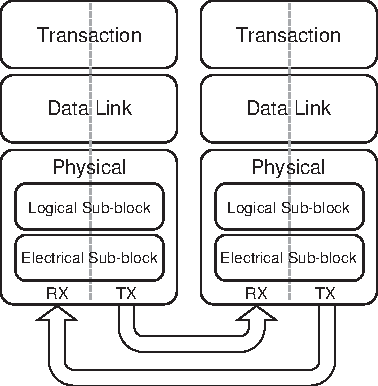
\includegraphics[width=0.5\textwidth]{pcie}
    \caption[PCI Express structure]{
        High-level diagram showing the layered structure of PCI Express. (Reprinted from \cite{pcie})
    }
    \label{fig:pcie}
\end{figure}

The transaction layer's primary responsibility is the creation and parsing of transaction layer packets (TLPs).
TLPs are used to trigger events or start various transactions, most commonly to initiate read and write requests\footnotemark.
\footnotetext{
    Read and write requests are directed at one of up to six base address registers (BARs).
    They represent internal memory areas that can be anywhere from a few bytes to several gigabytes in size.
}
Most requests entail the return of a completion TLP containing the requested data or other information.
TLPs consists of multiple 32-bit double words (DW), where the first is a common header describing the type of packet.

The data link layer ensures integrity by adding error detection codes to outgoing TLPs and performing error detection and correction on incoming TLPs.
It is also responsible for retransmission if corruption occurs.

The physical layer is responsible for serialization and deserialization of the data stream.
Each byte is padded with two extra bits (8b/10b encoding) to allow clock recovery.

%==============================================================================%

\section{Related Work}

\TODO

Format: Who? What? When? Main feature? Relation?

\subsection{CAM-8}

\begin{itemize}
    \item Cellular Automata Machine
    \item Semi-parallel CA simulator
    \item Indefinitely scalable 3D mesh-network multiprocessor
    \item Optimized for large inexpensive simulations
    \item Prototype faster than existing supercomputers
    \item Hope to whet the apetite of researchers with computing power
    \item Time-sharing of com resources interprocessor wires, allows scalability to be achieved with current tech
    \item Node: DRAM with millions of cells, SRAM look-up table
    \item Nodes update cells seqentially
    \item 3G site updates per second
    \item No traditional CA neighborhoods: Based on partitioning from lattice gas models (shifts bits around)
    \item Good at spatially moving data and interaction at lattice sites: Well suited for simulating physical systems using lattice-gas-like dynamics or localized interactions.
    \item Goal to bring computation closer to physics to improve computation
    \item Harness the astronomical computing power that is available in CA format
\end{itemize}

\subsection{CAM-Brain Machine}

\begin{itemize}
    \item FPGA based hardware that implements a GA to evolve CA based neural network with 1000 neurons in approx 1 second
    \item Part of CAM-Brain project: Goal to build a brain with 1 billion neurons
    \item New research field called "Brain Building"
    \item Up to 65K modules can be interconnected in a large RAM
    \item Modules are evolved and connected by human design
    \item Artificial brain with up to 70M neurons
    \item Updated at 130G cells per second. Enough for real-time robot control
    \item CoDi-1bit (Collect and Distribute), maybe more in future
    \item Spike Interval Information Coding: "spike train" to analog
    \item Hough Spiker Algorithm: Analog to "spike train"
    \item Goal to have 500 times faster update times compared to CAM-8 for (50-100 updates 10-20 times per second)
    \item Cells can be neuron, axon or dendrite
    \item Each module has 24x24x24 cells, can receive 1-bit signals from 188 other modules and send to 64640
    \item Neuron has 4-bit accumulator and threshold function, inputs can be subtractive
    \item Dendrites pass XOR of inputs
    \item Axons pass input to all others
    \item Dendrites and Axons grown interchangedly
    \item Signals representation: Custom convolution function (SIIC)
    \item "Function-level" evolvable hardware
    \item Cells have 6-bit register and other logic for com
    \item Each FPGA has 8x6x4 cells
    \item Fast reconfiguration (<1ms)of the FPGA between growth, signaling and genetic phases to save resources
    \item Controllable object to attract attention and be proof-of-consept: Robokitty
    \item "An assemblage of evolved CA based neural net modules"
\end{itemize}
